\documentclass[11pt]{article}
\usepackage{amsmath}
\usepackage{siunitx}
\usepackage{tikz}
\usepackage{graphicx}
\usepackage{longtable}
\usepackage{multirow}
\usepackage{adjustbox}
\usepackage{pifont}
\usepackage{ulem}
\usepackage{xcolor,colortbl}
\usepackage{pgfplots}
\usepackage{float}
\usepackage{amsmath}
\usepackage{listings}
\usepackage{hyperref}
\usepackage{graphicx}
\usepackage{subcaption}
\hypersetup{
    colorlinks=true,
    linkcolor=blue,
    filecolor=magenta,      
    urlcolor=cyan,
}
\usepackage{amsmath}
\usepackage{xepersian}
\settextfont{XB Niloofar}
\setlatintextfont{Linux Libertine O}
\setdigitfont{XB Niloofar}
\title{پاسخ سوالات تیوری پروژه‌ی مبانی بیو‌انفورماتیک}
\author{میلاد آقاجوهری ، احسان سلطان‌آقایی}
\begin{document}
\maketitle
در این مستند به بیان قسمت‌‌های عملی و برنامه‌‌نویسی قضیه می‌پردازیم. امکان نمایش این قسمت در Rmd برای ما وجود نداشت زیرا ما از سیستم makefile برای انجام کار‌های خود استفاده کرده‌ایم. دقت کنید که این سیستم بسیار حرفه‌ای و دقیق است. در واقع سیستم ما به صورت کامل اگر برای مثال یک خط از یک فایل تغییر کند تمام کارهای لازم برای بروزرسانی شدن نتایج را خود بخود انجام می‌دهد. کافیست که به پوشه‌ی Source بروید و دستور
\lr{make clean}
را بزنید تا تمام نتایج پاک شوند و سپس با زدن یک دستور ساده‌ی 
\lr{make all}
خواهید دید که تنها با استفاده از داده‌های ژنوم‌ها‌ی گونه‌ها و ماربرگ و ژن‌هایش تک تک نتایج یکی پس از دیگری ظاهر خواهند شد(حتی عکس‌ها). خود اجرا شدن این دستور در واقع یک مستند کامل از نحوه‌ی پیاده‌سازی این قسمت است اما آن رادر حال حاضر توضیه نمی‌کنیم زیرا ممکن است یک سری از کتابخانه‌هایی که در تولید نتایج استفاده کرده‌ایم در کامپیوتر شما موجود نباشد و دستور اجرا نشود و نتایج ناقص شوند اما می‌توانید پس از دیدن آن‌ها یکبار روند بالا را اجرا کنید و اگر مشکلی از لحاظ کتابخانه‌ها و میزان رم(بیش از چهار کافی است) پیش نیاید، از روند حاصل شدن نتایج لذت ببرید.
\section{یک توجه}
در این بخش ما تنها به توضیح بخش برنامه‌نویسی پرداخته‌ایم و از رسم نتایج خود‌داری کرده‌ایم. تمامی نتایج این بخش را می‌توانید در فایل pdf 
\lr{theoritical\_report.pdf}
ببینید که تمامی نتایج خواسته شده را با رسم تصاویر پوشش داده است.
\section{سخنی با خواننده}
می‌پذیریم که ارایه‌ی یک فایل پی‌دی‌اف و توضیح دادن یک فایل
makefile 
به جذابیت یک فایل Rmd نیست. اما فایل‌های makefile مزیت‌های زیادی دارند زیرا خودشان نحوه و روند اجرا شدن را ذخیره کرده‌اند و در صورت هر تغییری از آن‌جا شروع به به‌روز‌سانی تمام نتایج می‌کنند و تمام عکس‌ها و نمودارها را بروز میکندو ذخیره می‌کنند.اما به هر حال توضیح این روند در یک فایل پی‌دی‌اف جذابیت و گیرایی خاص یک Rmd را ندارد. از شما خواهش‌مندیم از فایل‌های موجود در بخش Data بازدید کنید که در زیر توضیح داده شده و البته نتایج حاصله را ببینید اگرچه در گزاریش بخش تیوری به صورت کامل آمده است.

\section{توضیح روند اجرای کد}
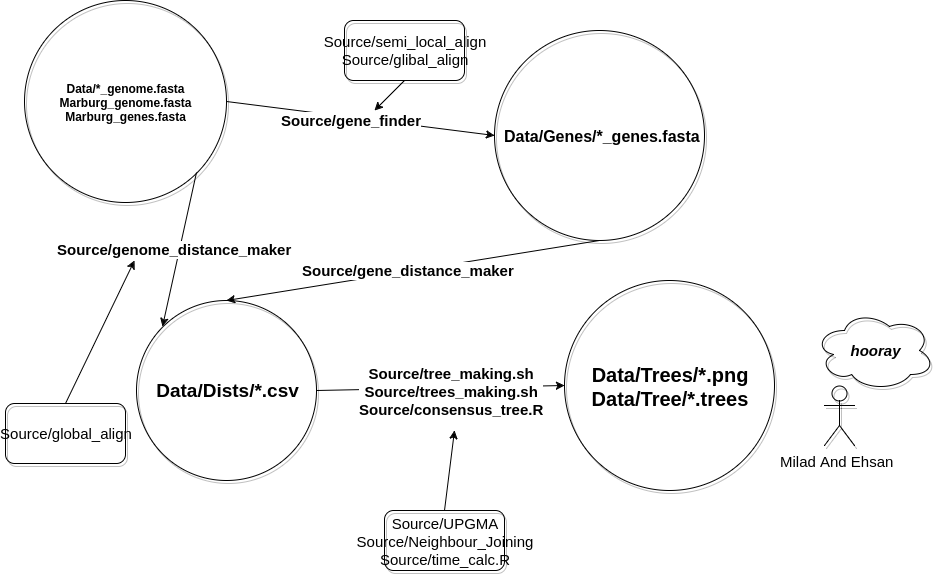
\includegraphics[scale = 0.5]{make_file.png}
در ابتدا ما تنها ژنوم ماربرگ و ژن‌های آن و در پوشه‌ی
\lr{Data/Genomes}
ژنوم گونه‌‌های ابولا را داریم.

 در این جا تکه کد
\lr{Source/gene\_finder.cpp}
اجرا می‌شود که با بارها استفاده از 
\lr{Source/semin\_local\_align.cpp}
هر ژن ماربرگ را در ژنوم ابولا سرچ می‌کندو نتایج را به ازای هر گونه از ابولا به نام مثلا X در 
\lr{Data/Genes/X\_gene.fasta}
می‌ریزد.

 سپس تکه کد
\lr{Source/gene\_distance\_maker.cpp}
از روی این فایل‌های ژن‌ها را خوانده و ماتریس فواصل را به دست آورده و در فایل‌هایی به نام 
\lr{Data/Dists/Y.csv}
میریزد که ماتریس حاصل از مقایسه برای ژنی به اسم مثلا Y است. 

 تکه کد
\lr{Source/genome\_distance\_maker.cpp}
از روی ژنوم فواصل بین ژن‌ها را به دست می‌آورد\newline و در 
\lr{Data/Dists/genome.csv}
میریزد.
 \newline
همین فواصل را به اضافه‌ی  ماربرگ در 
\lr{Data/Dists/all\_and\_marburg.csv}
میریزد.

 حال تکه کد 
\lr{Source/tree\_making.sh}
می‌آید و از روی 
\lr{Data/Dists/Y.csv}
 و با استفاده از 
 \lr{Source/UPGMA.cpp}
 , 
 \lr{Neighbour\_Joining.cpp}
 دو فایل 
 \lr{Data/Trees/Y\_UMPGA.png}
 و 
  \lr{Data/Trees/Y\_NJ.png}
  را میسازد. 
  
  
  در نهایت 
  \lr{Source/consensus\_tree.R}
  می‌آید و نتایج حاصل توسط
   \lr{UMPGA ,NJ} 
   را بهم ترکیب می‌کند و در قالب دو عکس
   \lr{Data/Trees/UMPGA.png}
 و 
  \lr{Data/Trees/NJ.png}
  در می‌آورد.
  
  
  برای بدست آوردن فاصله‌ی زمانی جدا شدن این‌گونه‌ها از هم کد 
  \lr{Source/time\_calc.R}
  با خواندن
  \lr{Data/Dists/all\_and\_marburg.csv}
  و فرمول گفته شده در بخش تیوری ماتریس فاصله‌ای بر حسب زمان‌ها به دست می‌آوریم و سپس از UPGMA از R استفاده می‌کنیم و درخت حاصل را به نام 
  \lr{Data/Tress/times.png}
  ذخیره می‌کنیم. در این جا تمام خواسته‌های پروژه انجام شده است.
 
\section{قسمت دوم}
\subsection{استخراج ژن ها}
ما در این قسمت از یک روش 
\lr{semi\_local\_alignment}
استفاده کرده‌ایم که کد آن در 
\lr{semi\_local\_alignment.cpp}
موجود است. این روش بهترین تطابق را ماتریس امتیازی که در آن شباهت امتیاز برابر با یک و تفاوت امتیاز -۱ و گپ امتیاز منفی یک دارد پیدا میکند
\lr{gap = -1, dif = -1, equal = +1}
 و یک dp ساده به صورت زیر است.
 \begin{latin}
 \begin{lstlisting}
 dp[i][j] = max(dp[i-1][j]+gap, dp[i][j-1]+gap, dp[i-1][j-1}
 +(genome[i]==gene[j]?equal:dif , if (j==0) 0)
 \end{lstlisting}
 \end{latin}
 است که البته جزییات در این کد ساده حذف شده است و میتوانید در خود فایل مشاهده کنید. اما قسمت آخر که اگر 
 $j = 0$
 بود می‌توانیم هزینه را صفر بگذاریم دلیلش این است که می‌توانیم قسمتی از اول ژنوم را بدون دادن هزینه مپ نکنیم و بیندازیم یعنی می‌توانیم فرض کنیم اول ژنوم بدون هزینه به گپ مپ شده است تا جایی که شروع کنیم به مپ کردن به ژن.
\subsection{هم‌ترازی ژن‌ها و به دست آوردن ماتریس فاصله}
برای به دست آوردن ماتریس‌های فاصله ابتدا باید کدی داشته باشیم که فاصله‌ي ویرایشی دو موجود را به ما خروجی بدهد. البته این کد به سادگی با تغییر در همان کد قسمت قبل حاصل می‌شود، کافیست ارفاق به ازای 
$j == 0$
را حذف کنیم و البته equal را نیز برابر صفر قرار دهیم. در این صورت فاصله‌ی ویرایش برابر با منفی یک ضربدر حاصل dpاست.
 \begin{latin}
 \begin{lstlisting}
 dp[i][j] = max(dp[i-1][j]+gap, dp[i][j-1]+gap, dp[i-1][j-1}
 +(genome[i]==gene[j]?0:dif)
 \end{lstlisting}
 \end{latin}
 این کد را در 
 \lr{global\_align.cpp}
 می‌توانید مشاهده کنید.
 سپس کدی داریم به نام 
 
 \lr{gene\_distance\_maker}
 که به ازای هر جفت ژن‌ها الگوریتم بالا را اجرا می‌کند و ماتریس را تشکیل می‌دهد(در این کد بسیار کدینگ زیبایی را شاهد هستیم، بین پروسه‌ها پایپ کرده‌ایم و غیره...).
\section{قسمت سوم}
\subsection{تشکیل درخت زندگی برای هر ژن}
دو الگوریتم UPGMAو NJ را الحمدلله قبلا در تمرین‌ها زده بودیم که از آن‌ها استفاده می‌کنیم و حاصل را توسط 
\lr{tree\_drawer}
می‌کشیم. کدینگ این قسمت در فایل 
\lr{tree\_making.sh}
موجود است و چندان نکته‌ي خاصی ندارد، صرفا دو برنامه‌ی ذکر شده اجرا و حاصلشان به 
\lr{tree\_drawer}
برای کشیدن داده می‌شود.


 \subsection{ترکیب درخت‌ها و ارائه‌ی درخت نهایی}
در اینجا از تابع 
consensus
از پکیج ape در آر استفاده کرده‌ایم. این تابع را صدا زده‌ایم و سپس حاصل را ذخیره کرده‌ایم. کدینگ این قسمت را در فایل
\lr{consesnsus\_tree.R}
میتوانید مشاهده کنید و لذت ببرید.
 \subsection{مقایسه‌ی درخت ترکیبی و درخت حاصل از همترازی سراسری}
 در این‌جا برای همترازی سراسری ما از همان کد خودمان که در بالا توضیح دادیم که فاصله‌ی ویرایشی محاسبه می‌کند استفاده کرده‌ایم. درخت ترکیبی حاصل هم در بالا توضیح دادیم که توسط 
 \lr{consesnsus\_tree.R}
 محاسبه می‌شود.
 
\subsection{تعیین نقطه‌ی شروع}
کد‌های لازم برای این قسمت در بقیه‌ی بخش‌ها توضیح داده شده است.
\section{بخش چهارم}
\subsection{چه زمانی از هم جدا شده‌اند؟}
قسمت‌های تیوری در گزارش بخش تیوری مشاهده شده است. در اینجا ما از روی فاصله‌هایی که در قبل حساب کرده‌ایم با استفاده از تکه کد
\lr{time\_calc.R}
آن‌ها را طبق فرمول گفته شده در بخش تیوری به ماتریس فاصله‌ی زمانی تبدیل و سپس از UPGMA استفاده کرده و در نهایت درخت حاصل را رسم و ذخیره می‌کنیم.
\end{document}

